\begin{question}{30}{
    Een luchtmacht onderzoekt de nauwkeurigheid van GPS-geleide raketten in een omgeving van elektronische oorlogsvoering.
    De raketten worden gericht op een vijandelijke luchtmachtbasis.
    Tijdens de vlucht worden de raketten ``gedesori\"enteerd'' omdat de vijandelijke troepen gebruik maken van GPS jammers om precisiewapens te verstoren.
    Onderzocht wordt nu wat het verband is tussen de afstand (in km) tussen de eerste locatie waar de raket gejamd wordt en het doelwit ($X$) en de afstand (in km) tussen het doelwit en het daadwerkelijke inslagpunt van de raket ($Y$).
    Van tien raketten worden data verzameld over deze twee variabelen.
    \begin{center}
        \begin{tabular}{c|cccccccccc}
            \toprule
                \textbf{$X$} & $30$ & $50$ & $70$ & $90$ & $110$ & $130$ & $150$ & $170$ & $190$ & $210$ \\
                \textbf{$Y$} & $3.9$ & $3.5$ & $2.7$ & $6.1$ & $4.4$ & $5.6$ & $6.3$ & $4.4$ & $8.1$ & $7.5$ \\
            \bottomrule
        \end{tabular}
    \end{center}

}

    \subquestion{4}{Teken de gegevens uit bovenstaande tabel in een spreidingsdiagram.} 
    \solution{
        \begin{center}
            \resizebox{0.9\textwidth}{!}{
                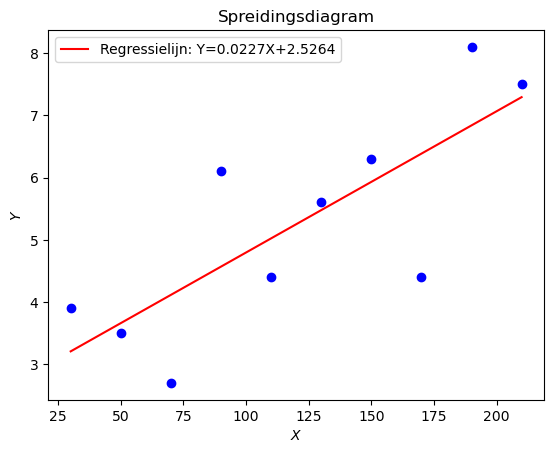
\includegraphics{opg2a.png}
            }
        \end{center}\rubric{4}
    }

    \subquestion{8}{Bereken met behulp van de tabel hierboven Pearson's correlatieco\"efficient. 
    Bepaal of er sprake is van een lineaire correlatie en leg in woorden uit wat de betekenis is van de grootte en het teken van de correlatieco\"efficient.
    }
    \solution{
        Hiervoor moeten we eerst een tabel uitschrijven met de grootheden $\overline{X}$, $\overline{Y}$, $\overline{XY}$, $\overline{X^2}$ en $\overline{Y^2}$.
            \begin{center}
                \begin{tabular}{ccccc}
                \toprule
                $X$ & $Y$ & $XY$ & $X^2$ & $Y^2$ \\
                \midrule
                $30$ & $3.9$ & $117$ & $900$ & $15.21$ \\
                $50$ & $3.5$ & $175$ & $2500$ & $12.25$ \\
                $70$ & $2.7$ & $189$ & $4900$ & $7.29$ \\
                $90$ & $6.1$ & $549$ & $8100$ & $37.21$ \\
                $110$ & $4.4$ & $484$ & $12100$ & $19.366$ \\
                $130$ & $5.6$ & $728$ & $16900$ & $31.36$ \\
                $150$ & $6.3$ & $945$ & $22500$ & $39.69$ \\
                $170$ & $4.4$ & $748$ & $28900$ & $19.36$ \\
                $190$ & $8.1$ & $1539$ & $36100$ & $65.61$ \\
                $210$ & $7.5$ & $1575$ & $44100$ & $56.25$ \\
                \midrule
                $\overline{X} = 120$ & $\overline{Y} = 5.25$ & $\overline{XY} = 704.9$ & $\overline{X^2} = 17700$ & $\overline{Y^2} = 30.3590$ \\
                \bottomrule
                \end{tabular}
            \end{center}\rubric{4}

            De correlatieco\"efficient van Pearson is gelijk aan
            \begin{align*}
                r   &= \frac{\overline{XY} - \overline{X} \cdot \overline{Y}}{\sqrt{(\overline{X}^2 - \overline{X^2}) \cdot (\overline{Y}^2 - \overline{Y^2})}} \\
                    &= \frac{704.9 - 120 \cdot 5.25}{\sqrt{(120^2 - 17700) \cdot (5.25^2 - 30.359)}} \\
                    &= \frac{74.9}{96.065} \\
                    &\approx 0.7797.
            \end{align*}\rubric{3}
            
            Deze correlatieco\"efficient duidt op een sterk positieve correlatie, oftewel wanneer een raket van grotere afstand gejamd wordt zal de raket ook verder van zijn doelwit inslaan.\rubric{1}
    }

    \subquestion{8}{Bereken de regressielijn $Y = aX + b$ met behulp van de tabel hierboven, en geef de interpretatie van $a$ en $b$ aan in dit scenario.}
    \solution{
        De co\"effici\"enten $a$ en $b$ van de regressielijn kunnen worden berekend aan de hand van twee vergelijkingen.
        Allereerst hebben we
        \[
            a = \frac{\overline{XY} - \overline{X} \cdot \overline{Y}}{\overline{X^2} - \overline{X}^{2}} = \frac{704.9 - 120 \cdot 5.25}{17700 - 120^2} \approx 0.0227 \rubric{3} 
        \]        
        Vervolgens geldt dan dat 
        \[
            b = \overline{Y} - a\cdot \overline{X} = 5.25 - 0.0227 \cdot 120 \approx 2.5264 \rubric{2}
        \]
        De regressielijn behorende bij deze steekproef is dus gelijk aan $Y = 0.0227X+2.5264$.\rubric{1}
        
        Je kunt deze regressielijn interpreteren als volgt: voor elke km dat de raket verder van het doelwit af jamming ervaart, zal de afwijking van de raket ten opzicht van het doelwit stijgen met $0.0227$ km.
        Verder is in het geval van geen jamming de afstand tussen doelwit en inslagpunt $2.5264$ km (bijvoorbeeld door weersfenomenen of rekenfouten tijdens lancering).\rubric{2}
    }

    \subquestion{2}{Geef een statistisch verantwoorde voorspelling van de afstand tot het doelwit waarop een raket inslaat die op $45$ kilometer van het doelwit voor het eerst GPS jamming ondervindt.}
    \solution{
        Je kunt de zojuist uitgerekend regressielijn gebruiken om een voorspelling te vinden.\rubric{1}
        Vul in $X = 45$, dit geeft $Y = 0.0227\cdot 45 + 2.5264\approx 3.5477$ km. \rubric{1}
        De raket zal naar verwachting zo ongeveer op iets meer dan 3.5 km van het doelwit inslaan.
    }

    \subquestion{8}{Bepaal een $95\%$-voorspellingsinterval voor de afstand tussen doelwit en inslagpunt als die op $120$ kilometer van het doelwit voor het eerst GPS-jamming ondervindt.}
    \solution{
            Het voorspellingsinterval is $[Y_{0} - t\cdot s_{f}; Y_{0} + t\cdot s_{f}]$, waarbij $Y_0 = 3.5477$ de puntschatting gemaakt bij de vorige opgave.
            Verder geldt dat $t$ de $t$-waarde is die hoort bij een betrouwbaarheid van $95\%$ met $df = n-2 = 10 - 2 = 8$ vrijheidsgraden. \rubric{1}
            Bij een betrouwbaarheid van $95\%$ is de linkeroverschrijdingskans $0.95+0.05/2 = 0.975$ en 
            \[
                t = \invt(opp=0.975; df=8) \approx 2.3060
            \]
            \rubric{1}
            Verder geldt voor de standaardafwijking van de errorterm:
            \begin{align*}
                s_{\epsilon}    &= \sqrt{\frac{n}{n-2}\cdot (\overline{Y^2} - a\cdot\overline{XY} - b \cdot \overline{Y})} \\
                                &= \sqrt{\frac{10}{8}\cdot (30.3590 - 0.0227\cdot 704.9 - 2.5264 \cdot 5.25)} \\
                                &\approx 1.0963
            \end{align*}
            \rubric{2}
            Verder geldt
            \begin{align*}
                u   &= \frac{1}{n} \cdot (1 + \frac{(X_0 - \overline{X})^2}{\overline{X^2} - \overline{X}^2}) \\
                    &= \frac{1}{10} \cdot (1 + \frac{(45 - 120)^2}{17700 - 120^2}) \\
                    &\approx 0.2705
            \end{align*}
            \rubric{2}
            De standaardafwijking van de forecasting term is dan
            \[
                s_{f} = s_{\epsilon} \cdot \sqrt{u+1} \approx 1.2357
            \]
            \rubric{1}
            Dit levert een interval op van $[Y_{0} - t\cdot s_{f}; Y_{0} + t\cdot s_{f}] = [0.6982; 6.3972]$.
            \rubric{1}
            Merk op dat dit interval zeer onnauwkeurig is en laat zien dat de voorspellende waarde van de regressielijn zeer beperkt is.
    }

\end{question}